\section{تصویر برداری موازی}

در این قسمت برای سرعت بخشیدن به فرایند تصویربرداری \mri روش هایی معرفی می‌شود که به تصویر برداری موازی 
\LTRfootnote{Parallel Imaging}
موسوم هستند.
در تصویربرداری \mri دادگان مستقیما از تصویر برداشته نمی‌شوند بلکه از فضای فوریه ‌ی تصویر موسوم به \kspace اخذ می‌شوند. (شکل \ref{fig:kspace-fov-res})






\begin{figure}[t!]
	\centering
	\begin{RTLcopyrightBox}{\linewidth}{\doiSource{10.1002/jmri.23639}}
		\subfigure[میدان دید کامل و رزولوشن کامل]{
			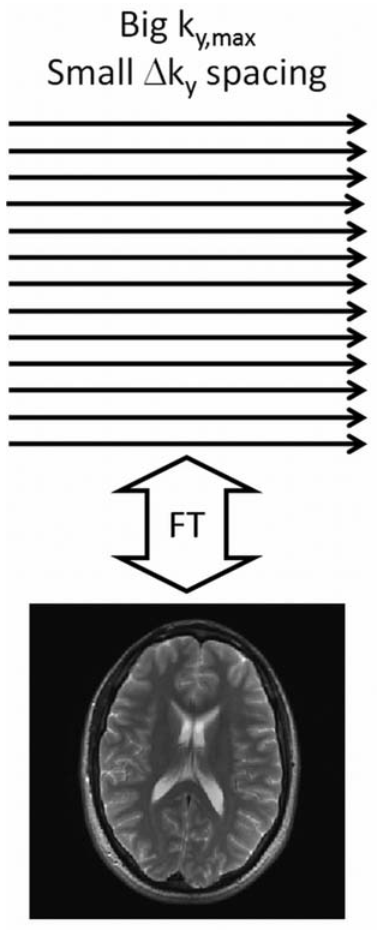
\includegraphics[width=0.3\linewidth]{chapters/chapter-3/figs/kspace-full-fov-full-res}
			\label{subfig:kspace-full-fov-full-res}}
		\hfill
		\subfigure[میدان دید کامل و رزولوشن کمتر]{
			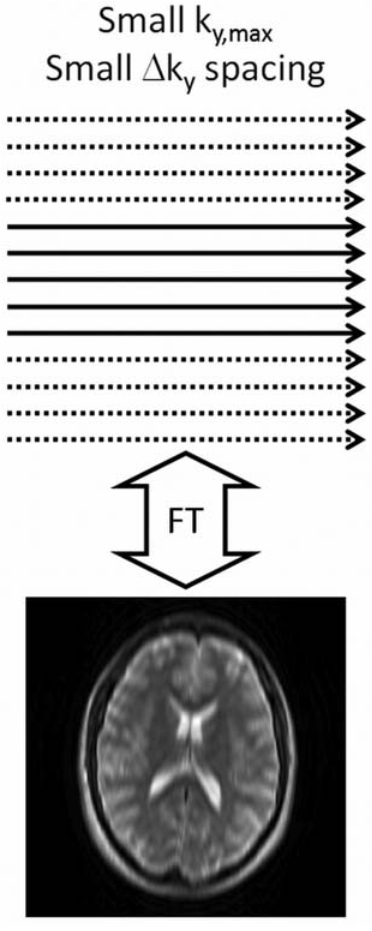
\includegraphics[width=0.3\linewidth]{chapters/chapter-3/figs/kspace-full-fov-lower-res}
			\label{subfig:kspace-full-fov-lower-res}}
		\hfill
		\subfigure[میدان دید کمتر و رزولوشن کامل]{
			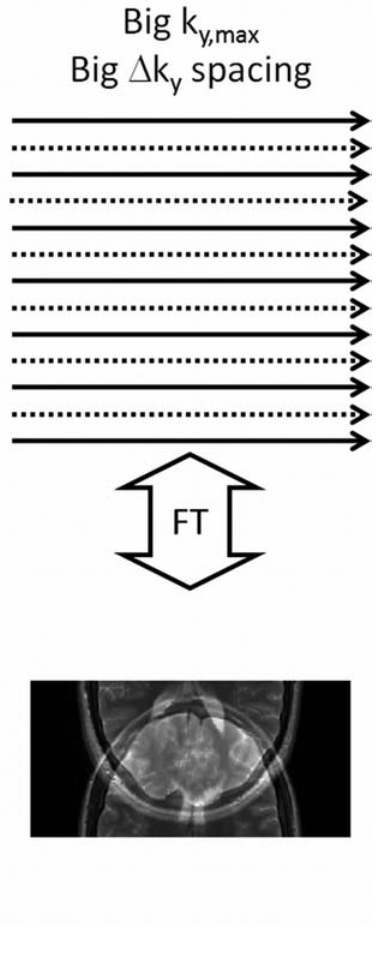
\includegraphics[width=0.3\linewidth]{chapters/chapter-3/figs/kspace-smaller-fov-full-res}
			\label{subfig:kspace-smaller-fov-full-res}}
		\hfill
	\end{RTLcopyrightBox}
	\removevspace
	\caption{}
	\label{fig:kspace-fov-res}
\end{figure}







سیگنال های بدست آمده عموما در جهت $k_x$ به صورت فرکانسی کد می‌شوند و در جهت $k_y$ به صورت خطوطی از کد کردن فاز می‌باشند. همچنین اگر تصویر برداری سه بعدی مدنظر باشد یک کد کردن دوم فاز نیز در جهت $k_z$ صورت می‌گیرد. زمان کل اخذ داده
\LTRfootnote{Total acqusition time}($T_A$)
برای یک اسکن دو بعدی به صورت زیر می‌باشد.

\removevspace
\begin{equation}
T_A = T_R \times N_{PE}
\end{equation}

که $T_R$ زمان تکرار
\LTRfootnote{Repetition time}
یا زمانی که نیاز است تا یک خط از \kspace در طول $k_x$ دریافت شود می‌باشد. همچنین $N_{\mathrm{PE}}$ نیز تعداد خطوط کد کردن فاز در جهت $k_y$ می‌باشد. در یک تصویر برداری سه بعدی، تعداد کد کردن پارتیشن ها
\LTRfootnote{Partition encoding}
($N_{\mathrm{PART}}$)
نیز باید به حاصل ضرب اضافه کرد.

$T_R$
کمک می‌کند که کنتراست تصویر را تنظیم کنیم و $N_{\mathrm{PE}}$
روزولوشن تصویر در جهت کدکردن فاز را تعیین می‌کند.

برای کاهش زمان استخراج داده، یا باید داده های \kspace سریع‌تر استخراج شود(که به معنی کاهش زمان $T_R$
است) و یا تعداد داده کمتری استخراج شود (که به معنای کاهش $N_\mathrm{PE}$ می‌باشد).


سرعت جمع آوری داده های \kspace، کنتراست مطلوب تصویر را تنظیم می‌کند. برای بعضی از انواع اسکن مانند اسپین اکو
\LTRfootnote{Spin Echo}
، $T_R$ باید به اندازه ای باشد تا کنتراست مطلوب تصویر تولید شود. در باقی انواع اسکن مانند 
گرادیان
\LTRfootnote{Spoiled Gradient Echo}
یا سری‌های تقدیمی آزاد حالت ماندگار متعادل
\LTRfootnote{Balanced Steady-State Free-Precession Sequences}
، کاهش زمان $T_R$ با حفظ کنتراست تصویر ممکن است.

اما یک محدودیت فیزیکی نیز وجود دارد. قطع و وصل کردن سریع گرادیان با میدان قوی می‌تواند یک جریان الکتریکی در بدن بیمار القا کند که آن نیز می‌تواند بالقوه باعث ایجاد تحریکات عصبی حاشیه‌ای
\LTRfootnote{Peripheral Nerve Stimulation}
 شود\cite{ParallelMRImaging2012}.

دیدگاه دیگر برای کاهش زمان $T_A$، کاهش تعداد داده های جمع آوری شده می‌باشد. یک راه برای این کاهش، کاهش ساده‌ی $k_{y, \max}$
می‌باشد در حالی که فاصله‌ی $\Delta k_y$ حفظ شده است (شکل \ref{subfig:kspace-full-fov-lower-res}).
از آن جا که طبق رابطه \ref{eq:fov-res-kspace}
رزولوشن در جهت $y$ با معکوس $k_{y,\max}$ متناسب است، این کار باعث کاهش رزولوشن تصویر و مات شدن آن می‌شود.
اگر رزولوشن تصویر بخاطر مسایل کلینیکالی بخواهد ثابت بماند، یک راه آن است که مانند شکل \ref{subfig:kspace-smaller-fov-full-res} برخی از خطوط کدکردن فاز حذف شوند. با این کار $\Delta k_y$ زیاد می‌شود و مطابق رابطه‌ی \ref{eq:fov-res-kspace} باعث کاهش در میدان دید تصویر می‌شود که درصورتی که ابعاد شئ از ابعاد میدان دید بزرگتر باشد، می‌تواند باعث ایجاد اختلاط مکانی
\LTRfootnote{Spatial Aliasing}
می‌شود. در حقیقت \lr{FOV} (که توسط فاصله‌ی خطوط کد کردن فاز تعیین می‌شود)، باید حداقل به بزرگی ابعاد شئ مورد تصویر برداری باشد. این الزام بر روی \lr{FOV} و محدوده‌ی نمونه برداری \kspace به عنوان نرخ نایکویست
\LTRfootnote{Nyquist criterion}
شناخته می‌شود. اگر نرخ نایکوییست در هردو جهت $k_x$ و  $k_y$ رعایت شود، تصویر می‌تواند مانند شکل \ref{subfig:kspace-full-fov-full-res}
بدون اختلاط مکانی بازسازی شود\cite{ParallelMRImaging2012}.



\subsection{روش های تصویربرداری موازی}

هنگامی که سرعت بخشیدن به جمع آوری داده های \mri با جمع آوری تعداد کمتری خطوط کدکردن فاز ممکن است که قبل از استفاده تصاویر در کاربرد های کلینیکی، اختلاط مکانی آن ها حذف شود. روش های تصویربرداری موازی در راستای حل کردن این مشکل، ایجاد شده اند. همه روش های تصویربرداری موازی سه مشخصه‌ی زیر را مشترک دارند\cite{ParallelMRImaging2012}:


\begin{figure}[t!]
	\centering
	\subfigure[]{
		\copyrightbox[b]{
			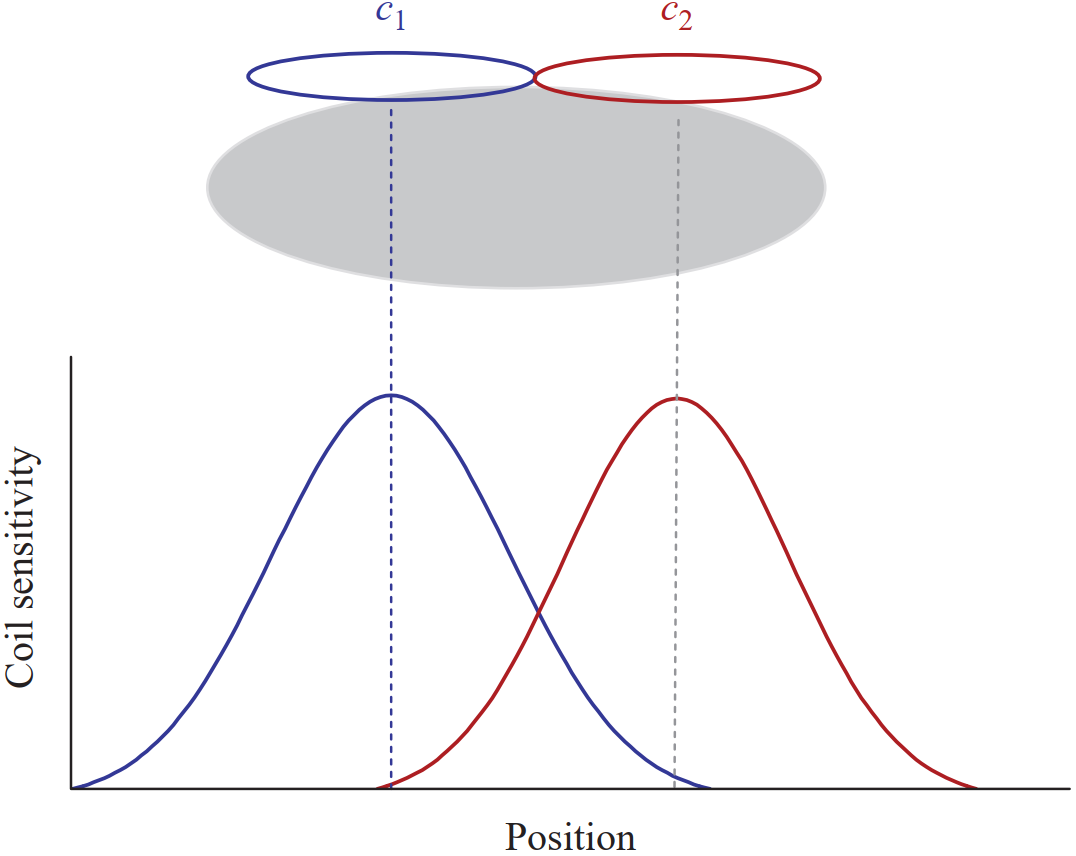
\includegraphics[width=0.45\linewidth]{chapters/chapter-3/figs/coil-sensivity-2}
			\label{subfig:coil-sensivity-2}
		}{\doiSource{10.1017/CBO9780511545405}}}
	\hfill
	\subfigure[]{
		\copyrightbox[b]{
			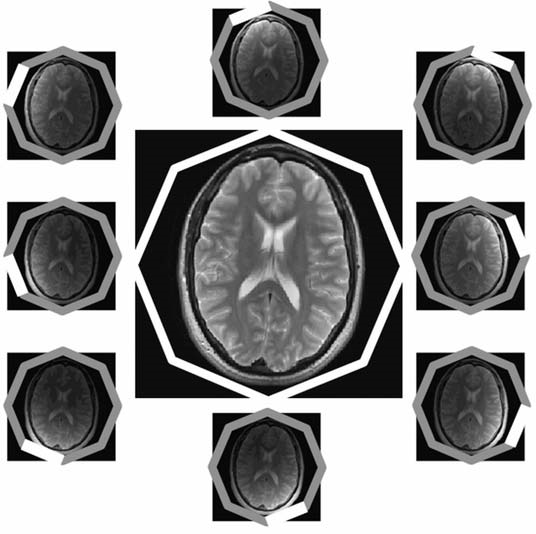
\includegraphics[width=0.36\linewidth]{chapters/chapter-3/figs/coil-sensivity-8}
			\label{subfig:coil-sensivity-8}
		}{\doiSource{10.1002/jmri.23639}}}
	\removevspace[1]
	\caption{}
	\label{fig:coil-sensivity}
\end{figure}



\removevspace[1]
\begin{enumerate}
	\item
	داده های \kspace در جهت کدکردن فاز برای کاهش زمان اسکن، زیر نرخ نمونه برداری شده اند (در تصویربرداری های سه بعدی می‌تواند در جهت کدکردن پارتیشن نیز چنین باشد).
	\textbf{فاکتور شتاب}
	\LTRfootnote{Acceleration factor}
	یا\textbf{ فاکتور کاهش}
	\LTRfootnote{Reduction factor}
	$R$ 
	به صورت نسبت مقدار دیتای \kspace برای نمونه برداری کامل تصویر به مقدار جمع آوری شده در یک استخراج تسریع یافته
	\LTRfootnote{Accelerated accqusition}
	، تعریف می‌شود. اگر نرخ نایکوییست رعایت نشود و میدان دید کمتر اندازه‌ی شئ باشد، تصویری دارای اختلاط را نتیجه می‌دهد.
	
	\item
	داده های بوسیله‌ی کانال‌های دریافت کننده ی مستقلی به جای یک سیم‌پیچ دریافت کننده همگن حجمی بزرگ (شکل \ref{subfig:coil-sensivity-8}) بدست می‌آیند. هریک از این سیم‌پیچ های دریافت کننده به حجمی که به آن‌ها نزدیک تر است حساس‌ترند.(شکل \ref{subfig:coil-sensivity-2})  که این یعنی که آن سیم‌پیچ ها یک منبع اضافه از اطلاعات مکانی جهت بازسازی تصویر را فراهم می‌کنند.

	\item
	یک الگوریتم مخصوص که به اطلاعات حساسیت سیم‌پیچ های مختلف برای بازسازی احتیاج دارد، برای ترکیب داده های زیر نرخ نمونه برداری شده از هر سیم‌پیچ دریافت کننده استفاده می‌شود تا یک تصویر نمونه برداری با میدان دید کامل بدون اختلاط بدست آید.
\end{enumerate}

چیزی که باید به آن توجه کرد این است که تصویربرداری موازی یک سری پالس خاص نیست.
تعداد کانال های دریافت کننده در آرایه ای از سیم پیچ ها، مقدار ماکسیمم فاکتور شتاب را محدود می‌کند.
\hl{به طور کلی، فاکتور شتاب نمی‌تواند از تعداد سیم‌پیچ های آرایه بیشتر شود. }
هرچند این پارامتر معمولا خیلی کمتر انتخاب می‌شود تا تصویری با کیفیت مطلوب تولید شود.

روش های مختلفی در تصویربرداری موازی وجود دارد و آن سه مشخصه‌ی مذکور بین‌شان مشترک است.این الگوریتم ها را می‌توان به دو دسته تقسیم کرد.
\begin{enuminline}
	\item آن‌هایی که با تصاویر دارای اختلاط  کار می‌کنند(مانند \lr{SENSE})	
	و 
	\item
	 آن‌هایی که داده های از دست رفته‌ی \kspace را بازسازی می‌کنند (مانند \lr{GRAPPA}).
\end{enuminline}

\subsection{آرایه های سیم‌پیچ های دریافت کننده}


قبل از بحث در مورد متود های مختلف تصویربرداری موازی مهم است که در مورد یک سخت افزار اساسی در تصویربرداری موازی یا به عبارت دیگر آرایه دریافت کننده چندکاناله
\LTRfootnote{multichannel receiver array}،
صحبت کرد.
حساسیت یک کانال دریافت کننده تکی در یک آرایه به سیگنال‌هایی که از یک منطقه مکانی خاص می‌آیند، محدود می‌شود که
در شکل \ref{fig:coil-sensivity}
قابل مشاهده است. این حساسیت معمولا به شئ درون سیم‌پیچ های دریافت کننده بستگی دارد و بنابراین از یک بیمار به بیمار دیگر می‌تواند تغییر کند. 

\begin{figure}[t!]
	\centering
	\copyrightbox[b]{
		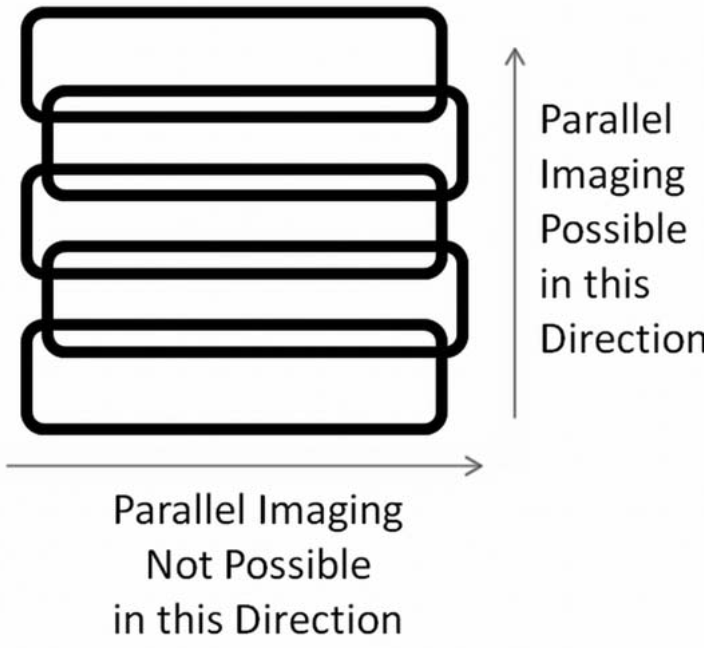
\includegraphics[width=0.4\linewidth]{chapters/chapter-3/figs/coil-sensivity-direction}
	}{\doiSource{10.1002/jmri.23639}}
	\removevspace[1]
	\caption{}
	\label{fig:coil-sensivity-direction}
\end{figure}

پروفایل های حساسیت، میدان دید مطلوب را پوشش می‌دهد. هنگامی که یک اسکن با چندین سیم پیچ دریافت کننده انجام می‌شود، تصاویر نتیجه شده از هر سیم‌پیچ باید با یکدیگر ترکیب شوند. این کار می‌تواند با استفاده از \textbf{مجموع مربعات} (و یا سایر تکنیک هایی که یک سیگنال همگن را پس از ترکیب نتیجه می‌دهند) انجام داد.

آرایه های متداول در  کاربردهای کلینیکالی از 4 تا بیشتر از 32 کانال مستقل را شامل می‌شود و حساسیت های متنوعی را در دو یا سه بعد دارند. از آنجایی که تصویربرداری موازی به این تفاوت های حساسیت سیم‌پیچ ها تکیه دارد، سرعت بخشیدن صرفا در جهت تغییرات حساسیت می‌تواند اعمال شود. برای مثال اگر پنج سیم پیچ مانند شکل
 \ref{fig:coil-sensivity-direction} 
در یک خط قرار گیرند، صرفا در جهت خط آرایه(جهتی که حساسیتی بین سیم پیچ ها تغییر می‌کند)، سرعت بخشیدن می‌تواند اتفاق بیفتد. \cite{ParallelMRImaging2012}



شکل \ref{fig:coil-sensivity-product}
که چگونه یک حساسیست ناهمگن سیم‌پیچ می‌تواند یک تصویر \mr را تغییر دهد. به زبان ریاضی، هر نقطه در تصویر شئ در نقطه متناظرش در نقشه حساسیت
\LTRfootnote{Sensivity Map}
ضرب می‌شود. بنابراین نقطه‌ A و B در تصویر سمت راست در شکل \ref{fig:coil-sensivity-product}
به ترتیب با $A=C_A \times I_A$ و $B=C_B \times I_B$ برابر هستند. بنابراین تصویر هر سیم‌پیچ برابر با ضرب تصویر شئ در نقشه‌ی حساسیت آن سیم پیچ می‌باشد.


\begin{figure}[t!]
	\centering
	\copyrightbox[b]{
		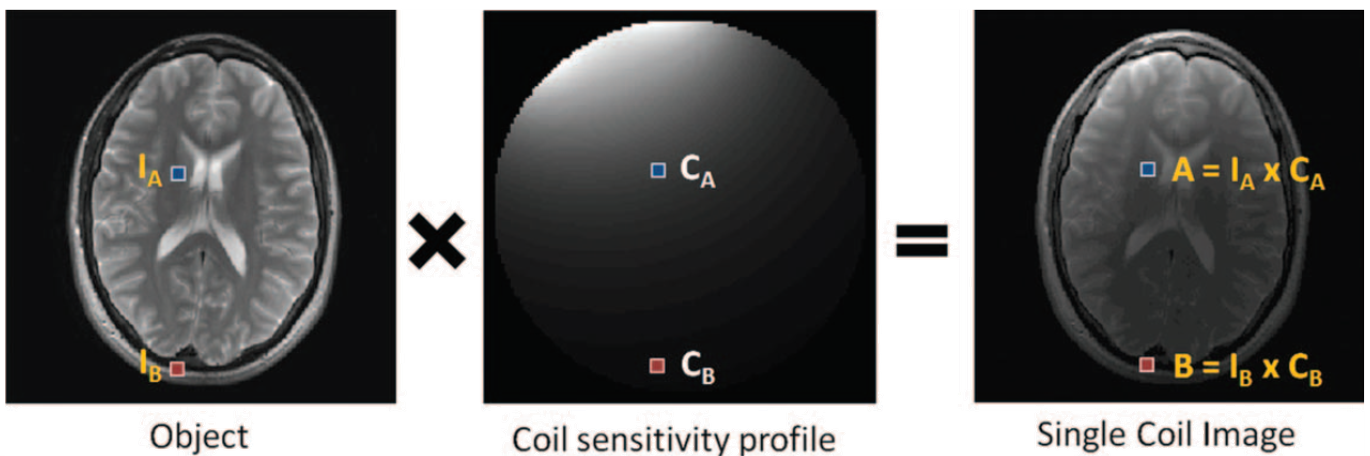
\includegraphics[width=0.9\linewidth]{chapters/chapter-3/figs/coil-sensivity-product}
	}{\doiSource{10.1002/jmri.23639}}
	\removevspace[1]
	\caption{}
	\label{fig:coil-sensivity-product}
\end{figure}






\subsection{تصویربرداری موازی جزئی با حساسیت های محلی شده(\lr{PILS})}


تصویربرداری موازی جزئی با حساسیت های محلی شده
\LTRfootnote{Partially Parallel Imaging With Localized Sensitivities}(\lr{PILS})

\cite{PILS-Griswold2000}

\begin{figure}
	\centering
	\copyrightbox[b]{
		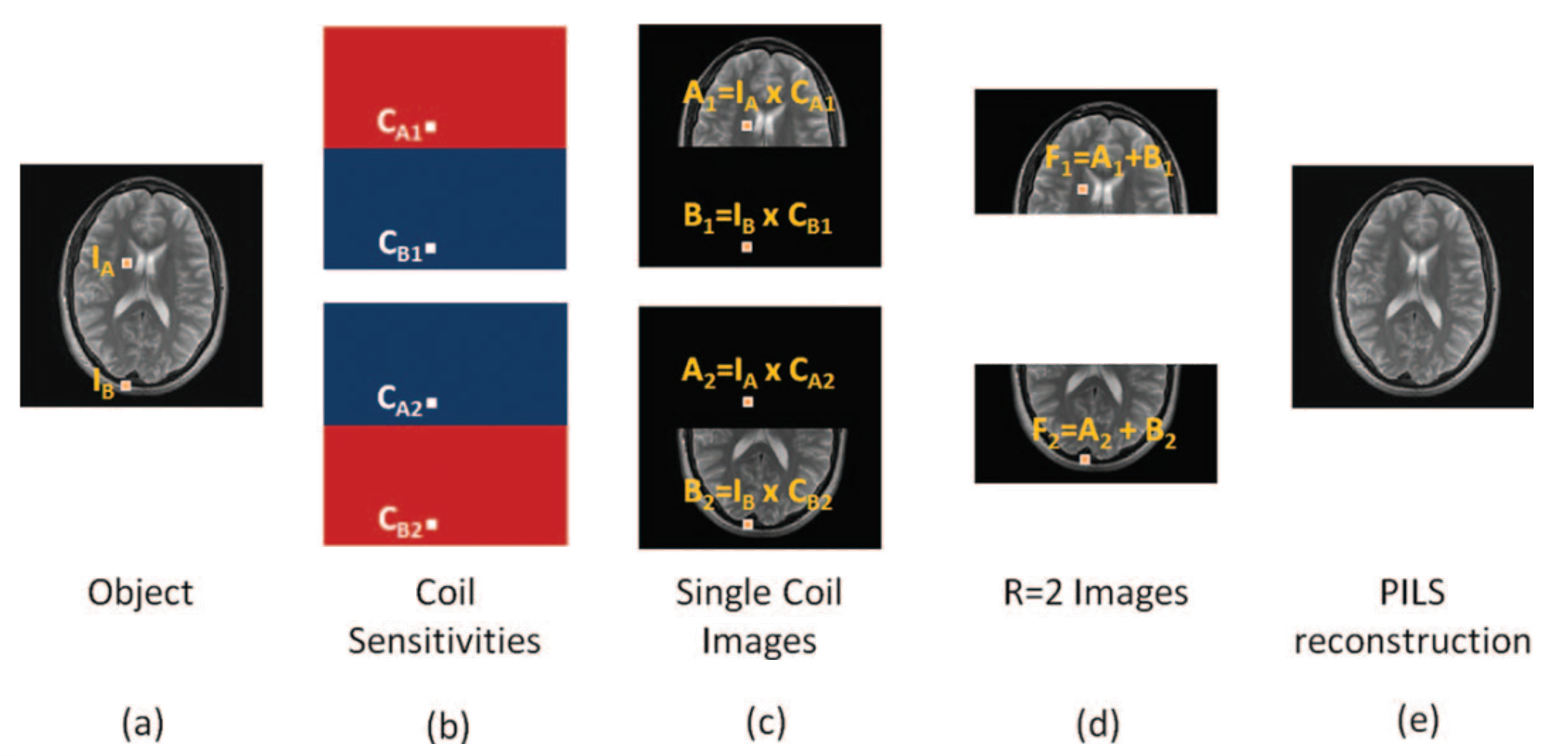
\includegraphics[width=0.8\linewidth]{chapters/chapter-3/figs/PILS-rec}
	}{\doiSource{10.1002/jmri.23639}}
	\removevspace[1]
	\caption{}
	\label{fig:pils-rec}
\end{figure}




\subsection{کدکردن حساسیت (\lr{SENSE})}

\LTRfootnote{SENSivity Encoding}(\lr{SENSE})
\cite{SENSE-1999}

\subsection{\lr{SMASH}}

\LTRfootnote{SiMultaneous Acquisition of Spatial Harmonics}(\lr{SMASH})

\subsection{\lr{GRAPPA}}

\LTRfootnote{Generalized Autocalibrating Partially Parallel Acquisitions}(\lr{GRAPPA})

\cite{GRAPPA-Griswold2002}








